\documentclass[aps,prl,reprint]{revtex4-1}
\usepackage{blindtext}

\usepackage{amsmath}
\usepackage{graphicx}
\usepackage{commath}
\usepackage{siunitx}
\usepackage{tabularx}

\usepackage{graphicx}


\usepackage[b]{esvect}

\newcommand{\de}{\mathrm{d}}

\graphicspath{ {images/} }
\begin{document}
\title{Unit 2: RC Circuits}
\author{Xueqi Li}
% \email{xueqi.li@stonybrook.edu}
\thanks{Partner: Tianming Hai}
% \author{partner Tianming Hai}
\noaffiliation
\date{Feb 17, 2018}


% \begin{abstract}
% Here I tell what I have done... And I have done a lot but it is hard to tell what exactly I have done...
% \end{abstract}

\maketitle

\section{Introduction}  
    \subsection{Capacitor}
    A capacitor can used to store change and voltage. Capacitance $C$ is defined as:
    \[
        C = \frac{Q}{V}
    \]
    
    For a sine wave input, for example, $V_\text{in} = V_0 e^{i\omega t}$, we can consider the capacitor as a resistor:
    \[
        Z_C = \frac{1}{i\omega C}
    \]
    The reason for that is $e^{i\omega t}$ is a eigenfunction for differential operation with eigenvalue $i \omega$. This imply that the solution of the differential equation would be a same function with a complex coefficients, which present the amplitude and the phase shift. Conister a pure capacitor circuits with a sine wave input, than one can have
    \[
    I = C \frac{\de V}{\de t} = C V_0 i \omega e^{i\omega t} = i \omega C V
    \]
    we see that $\frac{\de }{\de t} V= i \omega V$ as the pattern of eigenfunction. Now we can have the I-V relation:
    \[
    \frac{V}{I} = \frac{V}{i \omega C V} = \frac{1}{i \omega C} = Z_C
    \]
    Thus, it follows every rule for a resistor, such as series and parallel rules.
    \subsection{RC Circuits}
        A RC circuits is such a capacitor and the resistor in series. Thus, one can write following equations:
        \begin{equation}
            V_\text{in} = \frac{\de Q}{\de t} R + \frac{Q}{C}\label{eq:diffeq}
        \end{equation}
        where $I = \frac{\de Q}{\de t}$. One can solve this equation and find out the voltage and current in the circuits. However, for a sine wave input, we can use $Z_C$ to approch:
        \begin{align*}
            V_\text{in} &= V_0 e^{i \omega t} = IR + \frac{I}{i \omega C} \\
            I &= \frac{V_\text{in}}{Z_\text{tot}} = \frac{V_\text{in}}{R + \frac{1}{i \omega C}}
        \end{align*}
        If one wish to find the voltage in capacitor, it is possible to conclude by using the voltage divider equation:
        \[
        V_C = I Z_C = \frac{V_\text{in} \frac{1}{i\omega C}}{R + \frac{1}{i \omega C}} = \frac{V_\text{in} }{R i \omega C + 1}
        \]
        This lead to following solution:
        \begin{align}
            \abs{V_C} &= \frac{V_\text{in}}{\sqrt{1 + (\omega R C)^2}}; \nonumber\\
            \varphi &= \tan^{-1} \frac{\Im[V_C]}{\Re[V_C]} = \tan^{-1} (-\omega R C) \label{eq:lowpass}
        \end{align}
        where $\varphi$ is the phase shift.

        One can proceed the same calculation for voltage on resistor:
        \[
        V_R = I R =  \frac{V_\text{in} R}{R + \frac{1}{i \omega C}} = \frac{V_\text{in} R i \omega C}{R i \omega C + 1}
        \]
        and conclude the following solution:
        \begin{align}
            \abs{V_R} &= \frac{V_\text{in} \omega R C}{\sqrt{1 + (\omega R C)^2}} ; \nonumber\\
            \varphi &= \tan^{-1} \frac{\Im[V_R]}{\Re[V_R]} = \tan^{-1} (\frac{1}{\omega R C})\label{eq:highpass}
        \end{align}

    \subsection{Low Pass}
        \begin{figure}[h]
            \centering
            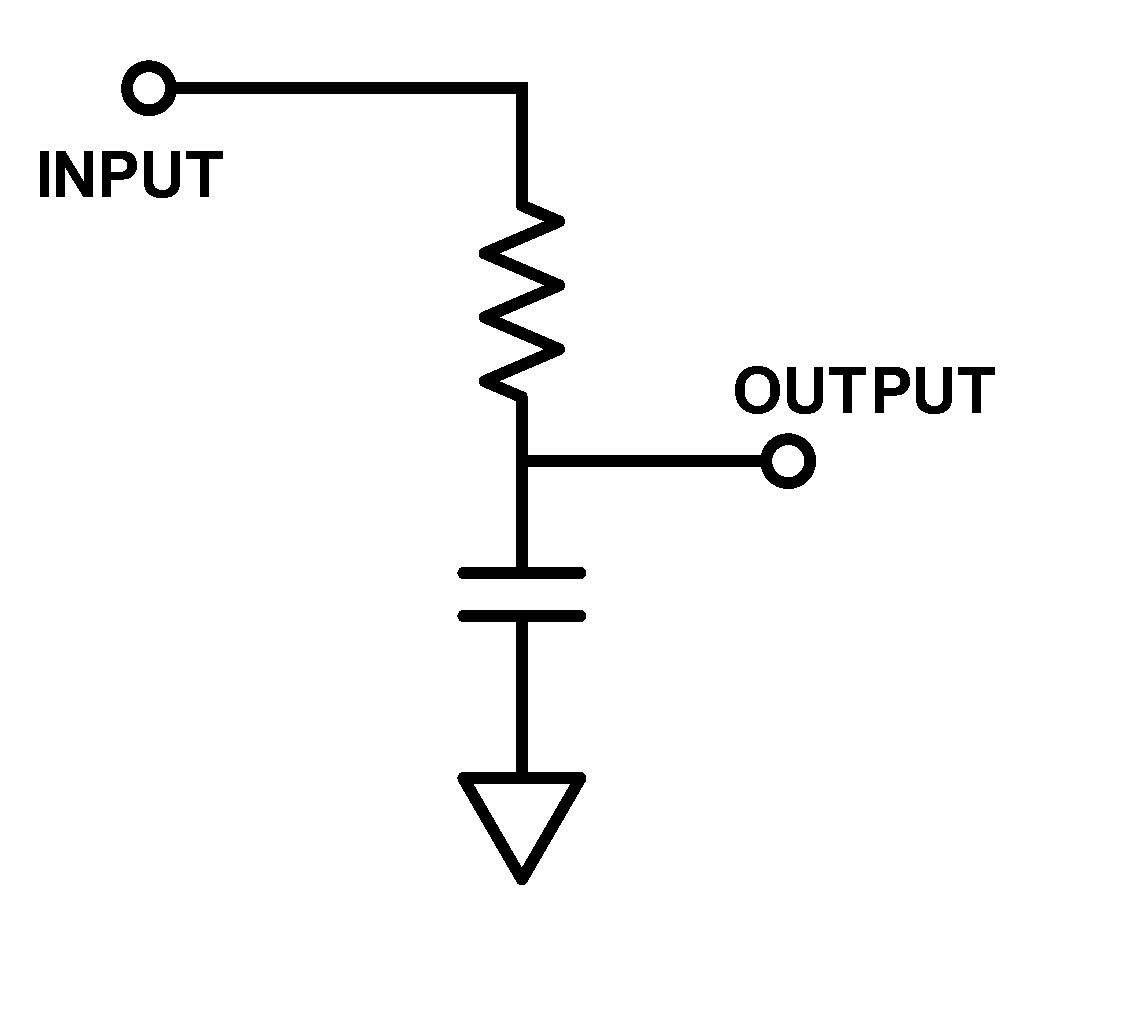
\includegraphics[width=1in]{image/lowpass.pdf}
            \caption{Low Pass}
            \label{fig:lowpass}
        \end{figure}
        A low pass is a RC circuits as above with the voltage on capacitor as the output, such as presented in Figure~\ref{fig:lowpass}. Using the Equation~\ref{eq:lowpass}, one take limit when $\omega R C \gg 1$:
        \[
        \abs{V_C} \approx \frac{V_\text{in}}{\omega R C}
        \]
        since $\omega$ is very large, than \abs{V_C} would be very small. One can also take the limit when $\omega R C \ll 1$:
        \[
        \abs{V_C} \approx V_\text{in}
        \]
        which is same as input voltage.

        There is such a case that $\omega R C = 1$:
        \[
        \abs{V_C} \approx \frac{V_\text{in}}{\sqrt{2}}
        \]
        Such point gives us the -3dB point:
        \[
        20 \log_{10} \frac{1}{\sqrt{2}} \approx -3\text{dB}
        \]
        Thus, at -3dB point, the output is around $0.71V_\text{in}$.

        One can approch same limit for the phase shift, but much easyer. When $\omega R C$ is high, we can have $\lim_{\omega R C \rightarrow \infty} \tan^{-1} (-\omega R C) = -\frac{\pi}{2}$. When $\omega R C$ is small, we can have $\lim_{\omega R C \rightarrow 0} \tan^{-1} (-\omega R C) = 0$. And when $\omega R C = 1$, we find $ \tan^{-1} (1) = -\frac{\pi}{4}$.

    \subsection{High Pass}
        \begin{figure}[h]
            \centering
            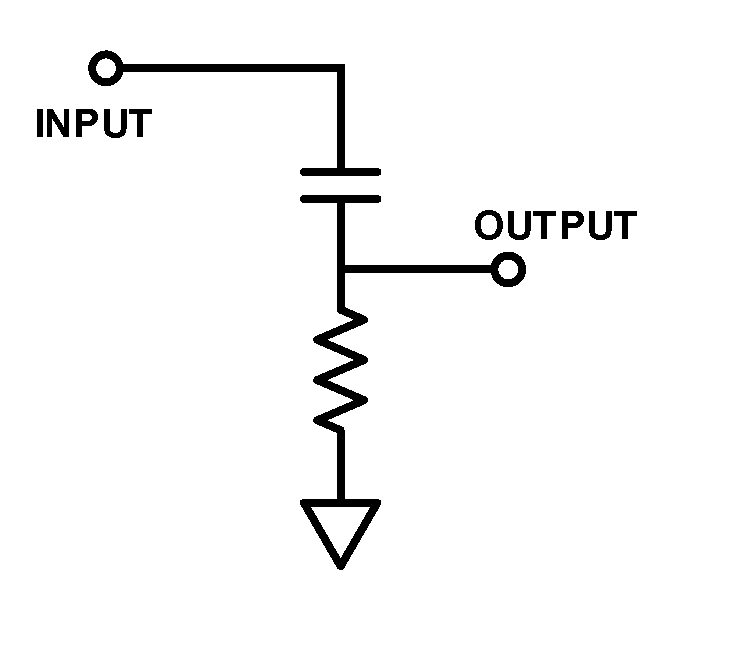
\includegraphics[width=1in]{image/highpass.pdf}
            \caption{High Pass}
            \label{fig:highpass}
        \end{figure}
        A high pass is a RC circuits such that it uses the voltage on resistor as output, presented in Figure~\ref{fig:highpass}. One can use the Equation~\ref{eq:highpass} to observe the result of the circuit. Take the same limit as low pass, following result can be obtained.
        \begin{align*}
            \abs{V_R} &= 
            \begin{cases}
                V_\text{in},                & \text{if } \omega R C \gg 1;\\
                \frac{V_\text{in}}{\sqrt{2}}, & \text{if } \omega R C = 1;\\
                V_\text{in}\omega R C,      & \text{if } \omega R C \ll 1\\
            \end{cases}\\
            \varphi &= 
            \begin{cases}
                \frac{\pi}{2},                & \text{if } \omega R C \rightarrow 0;\\
                \frac{\pi}{\sqrt{4}}, & \text{if } \omega R C = 1;\\
                0,      & \text{if } \omega R C \rightarrow \infty\\
            \end{cases}\\
        \end{align*}
    \subsection{Band Pass}
        \begin{figure}[h]
            \centering
            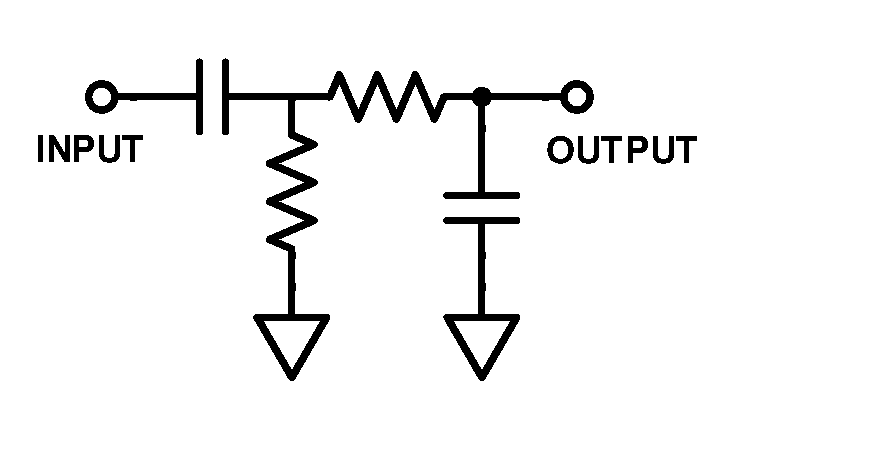
\includegraphics[width=1.5in]{image/bandpass.pdf}
            \caption{Band Pass}
            \label{fig:bandpass}
        \end{figure}
        One can connect the low and high pass together to form a band pass, such as Figure~\ref{fig:bandpass}. This will reduced the voltage with frequency both high or low with given capacitor and resistor. For example, if the high pass and low pass using same capacitor and resistor, the highest frequency remanind would be the -3dB point.

    \subsection{Differentiator}
        If the input voltage is not a sine wave, one must either consider the input voltage as a Fourier series of sine wave or solve the differential equations as Equation~\ref{eq:diffeq} directly. For example, one can find the voltage in resistor as:
        \[
        V_R = \frac{\de Q}{\de t}R = \frac{\de V_CC}{\de t}R = \frac{\de V_C}{\de t}RC
        \]
        That is to say, for a high pass, the output is the derivative of the voltage on capacitor. If the voltage on capacitor is close to the input voltage, which is the case for low frequency, this form a differentiator.
\section{Data and Calculation}
    In this experiment, we wish the -3dB point is between one and two kHz. Using the Equation~\ref{eq:lowpass}, we find following:
    \begin{equation}
        f_\text{-3\text{dB}} = \frac{1}{2\pi RC} \label{eq:findingfrequency}
    \end{equation}
    In here, we chose a $1.10(1)\text{k}\Omega$ (uncertainty measure from the minmum digit of the MMD) resistor and a $0.089(15)\mu$F (uncertainty measure from the chinging digits of the capacitance measuring instrument). Using Equation~\ref{eq:findingfrequency}, we expect the -3dB point is around $1.77(7)$kHz. The high pass and the low pass using the same RC combination. Using Equation~\ref{eq:highpass} we found the -3dB point is same as the low pass case, i.e., follow the Equation~\ref{eq:findingfrequency}. The input voltage amplitude in this section is 1V and has been adjust to 1V before every single measurement.

    \subsection{Low Pass}
        \begin{figure}[h]
            \centering
            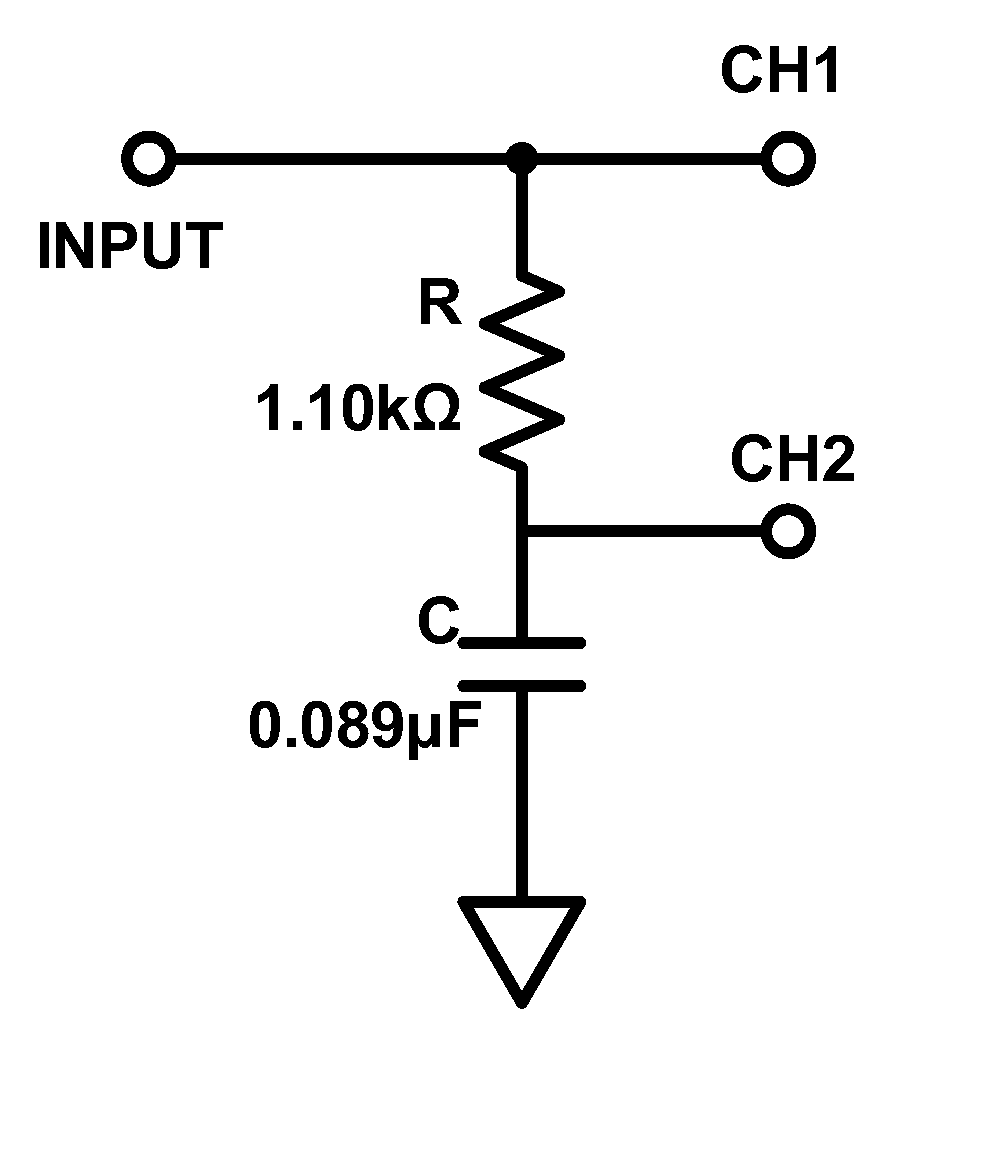
\includegraphics[width=1in]{image/lowpasslab.pdf}
            \caption{Circuit used for the low pass in lab}
            \label{fig:lowpasslab}
        \end{figure}

        We form the circuit as in Figure~\ref{fig:lowpasslab} in the lab. Please reference to the appendix for the obtained data. 
        \begin{figure}[h]
            \centering
            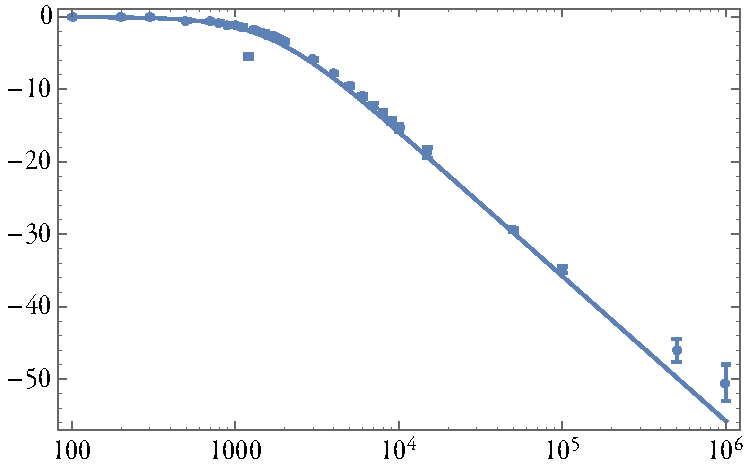
\includegraphics[width=3in]{image/lowpassvplot.pdf}
            \footnotetext{Some error bars might too small to see}
            \caption{The experiment data for output voltage of a low pass ($V_\text{out}$[dB] v. $f$[Hz])}
            \label{fig:lowpassvplot}
        \end{figure}
        \begin{figure}[h]
            \centering
            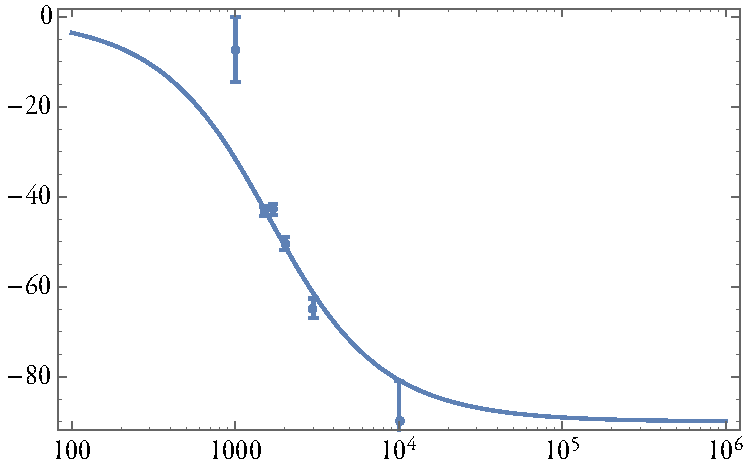
\includegraphics[width=3in]{image/lowpasspplot.pdf}
            \footnotetext{Some error bars might too small to see}
            \caption{The experiment data for output phase of a low pass (degree v. $f$[Hz])}
            \label{fig:lowpasspplot}
        \end{figure}
        Using the Equation~\ref{eq:lowpass}, we can also find the Theoretical value for output. Thus, a plot as Figure~\ref{fig:lowpassvplot} and Figure~\ref{fig:lowpasspplot} can be obtained.

    \subsection{High Pass}
        \begin{figure}[h]
            \centering
            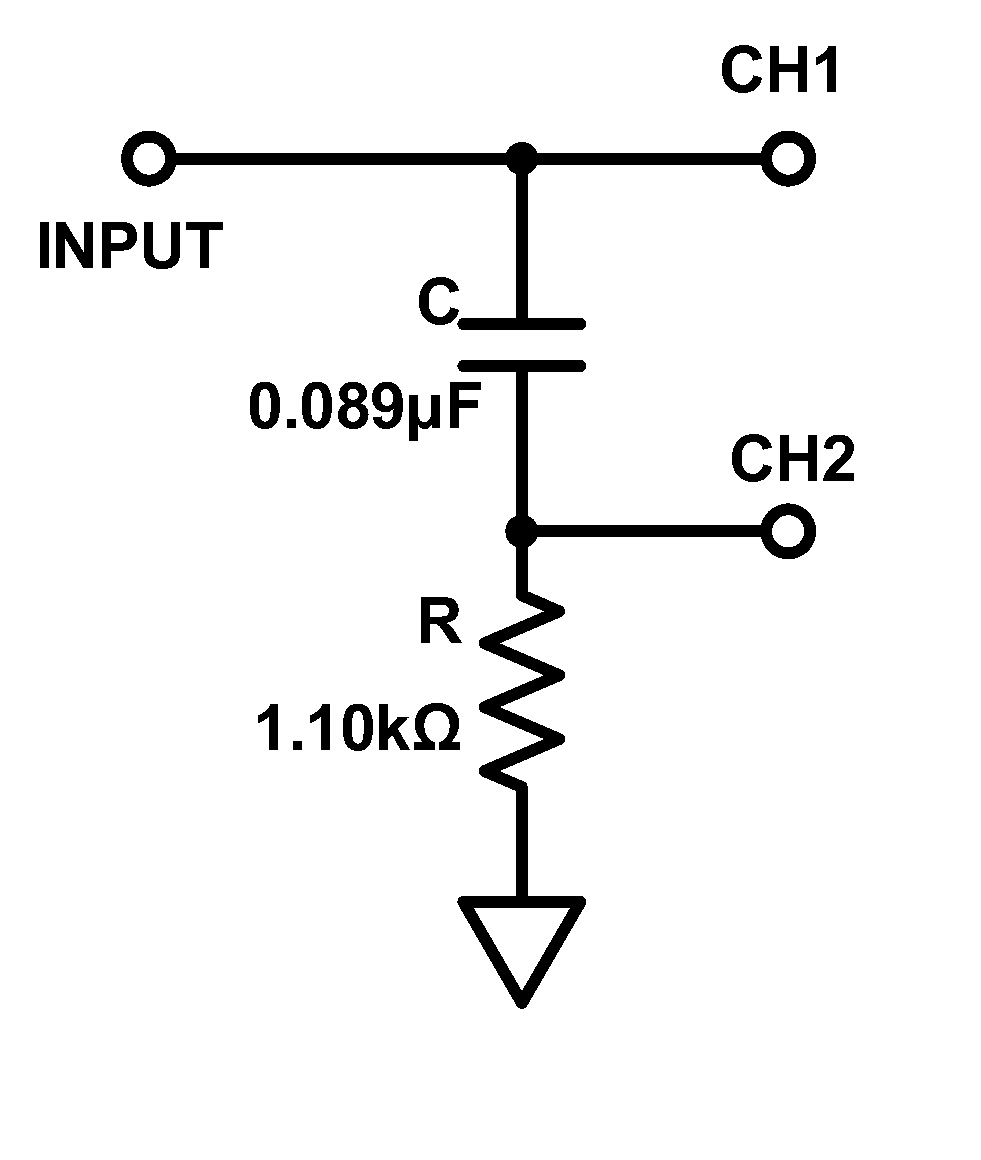
\includegraphics[width=1in]{image/highpasslab.pdf}
            \caption{Circuit used for the high pass in lab}
            \label{fig:highpasslab}
        \end{figure}
        We form the circuit as in Figure~\ref{fig:highpasslab} in the lab. Please reference to the appendix for the obtained data.
        \begin{figure}[h]
            \centering
            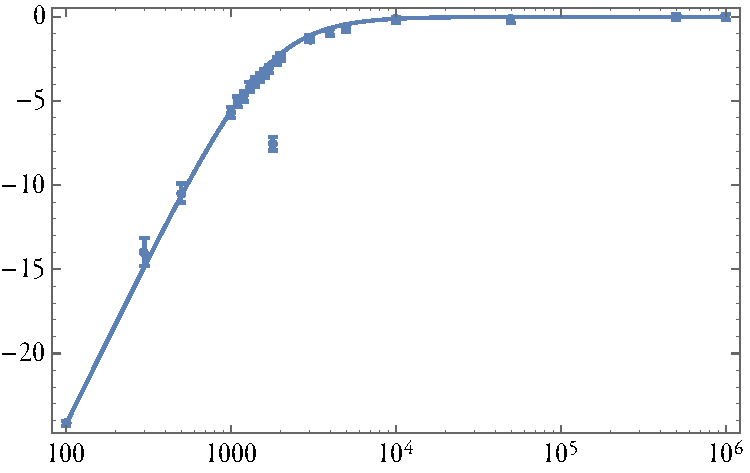
\includegraphics[width=3in]{image/highpassvplot.pdf}
            \footnotetext{Some error bars might too small to see}
            \caption{The experiment data for output voltage of a high pass ($V_\text{out}$[dB] v. $f$[Hz])}
            \label{fig:highpassvplot}
        \end{figure}
        \begin{figure}[h]
            \centering
            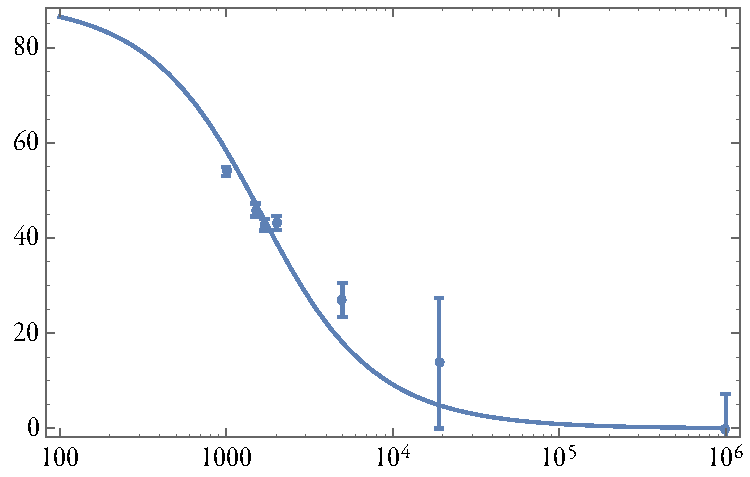
\includegraphics[width=3in]{image/highpasspplot.pdf}
            \footnotetext{Some error bars might too small to see}
            \caption{The experiment data for output phase of a high pass (degree v. $f$[Hz])}
            \label{fig:highpasspplot}
        \end{figure}
        Using the Equation~\ref{eq:highpass}, we can also find the Theoretical value for output. Thus, a plot as Figure~\ref{fig:highpassvplot} and Figure~\ref{fig:highpasspplot} can be obtained.

        When in low frequency, we obtained the result of a differentiator. Please reference to appendix for the picture of differentiator.

    \subsection{Band Pass}
        \begin{figure}[h]
            \centering
            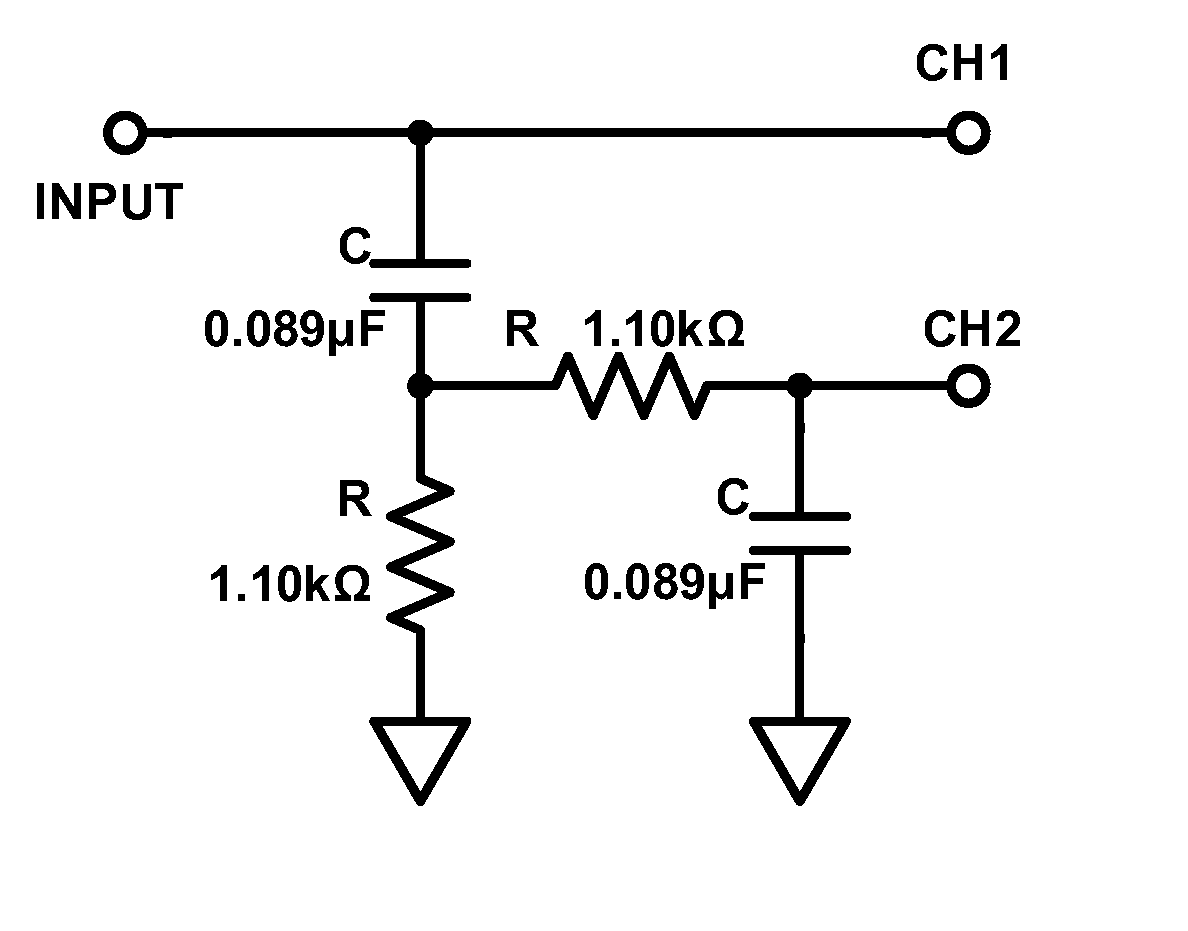
\includegraphics[width=1.5in]{image/bandpasslab.pdf}
            \caption{Circuit used for the band pass in lab}
            \label{fig:bandpasslab}
        \end{figure}
        \begin{figure}[h]
            \centering
            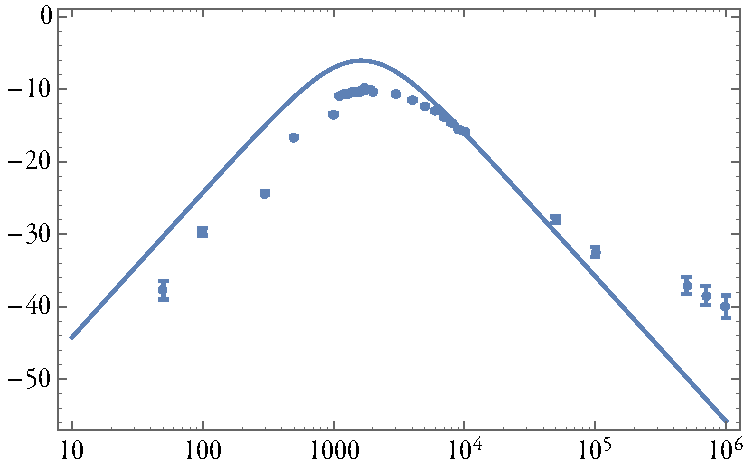
\includegraphics[width=3in]{image/bandpassplot.pdf}
            \footnotetext{Some error bars might too small to see}
            \caption{The experiment data for output voltage of a band pass ($V_\text{out}$[dB] v. $f$[Hz])}
            \label{fig:bandpassvplot}
        \end{figure}
        We form the circuit as in Figure~\ref{fig:bandpasslab} in the lab. Please reference to the appendix for the obtained data. The experiment data is as Figure~\ref{fig:bandpassvplot}.

\section{Analysis}
    \subsection{Low Pass}
        The reasult is reasonable. In low frequency, except one data point, all other data point are on the theoretical curve or within the error bar. At -3dB point, we expect to see 710mV in that point, which is discussed in introduction. In the experiment, we do observe such amplitude within around 1.77(7)kHz within $1\sigma$. The -3dB point is same as expect. The high frequency datapoint is higher than the theoretical result. The result is within $2\sigma$. Consider in high frequency, the voltage is very samll (less than 5mV), there might be other background noise interfered the result.

        The result of phase is also reasonable, in frequency higher than 1kHz, the result is within $1\sigma$. However, in frequency smaller than 1kHz, the result is about $2\sigma$ away from the theoretical value. It is true that in low frequenct the phase shift is much harder to measure since the center of the peak is difficult to identify, so as any other part of the sine wave. This might be an error on measurement.
    \subsection{High Pass}
        The reasult is reasonable. Except one data point, all other point are on the theoretical curve or within the error bar. We observe 710mV around 1.77(7)kHz within $1\sigma$. This is a high pass with expected -3dB point.

        The result of phase is also reasonable, most of the data point are within $1\sigma$ of the theoretical curve. There are two data points are within $2\sigma$ of the theoretical curve.

        When low frequency, we observe it is a differentiator. For a square wave, we obtained an output of a set of delta function, which is the derivative of the square wave, and when input frequency is a triangle wave, we obtained the result as a square wave, which is the derivative of the triangle wave. We see that once the frequenct are above 100Hz, the result is starting to becomming worse, once the frequenct are above 300Hz, the result is not very useful, but can still identify the rough shape.

    \subsection{Band Pass}
        The output reached its maximum around 1.77(7)kHz within $1\sigma$, so as the theoretical value. This is reasonable. However, the amplitude obtained around the maximum are smaller than the theoretical value. Moreover, other data point seems are a little bit tilt to the left: The lower frequency are smaller than the theoretical value and the higher frequency are higher than the theoretical value. That is to say, there is soemthing reduced the lower frequenct further but enhanced the higher frequency.

\section{Conclusion}
    The experiment is successful on high and low pass, but there measurement on phase shift can be strengthen. The result of band pass is interesting. Since the maximum achieve as expect, that means it is a band pass with the expect construction (same -3dB point high and low pass at 1.77Hz); however, the reason of the tilting needs to be researched farther.

\bibliography{cite}
\bibliographystyle{apsrev4-1}

    % \begin{figure}[h]
    %     \centering
    %     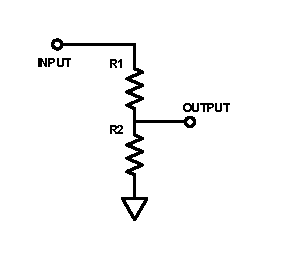
\includegraphics{images/plot2.pdf}
    %     \caption{A voltage divider}
    %     \label{fig:2}
    % \end{figure}

    % \begin{table}[h]
    % \begin{ruledtabular}
    % \begin{tabular}{cccc} 
    % Load[k$\Omega$] &  Output Voltage[V] & $R_\text{th}[\Omega]$ & Theoretical Voltage\\ \hline\hline
    % 50              & 0.680(1)           & 501(1)                & 0.682 \\ \hline
    % 500             & 3.75(1)            & 500(1)                & 3.75 \\ \hline
    % 5000            & 6.80(1)            & 514(1)                & 6.82 \\
    % \end{tabular}
    % \end{ruledtabular}
    % \caption{Load resistor and the output}
    % \label{table:8}
    % \end{table} 

% \begin{center}
%  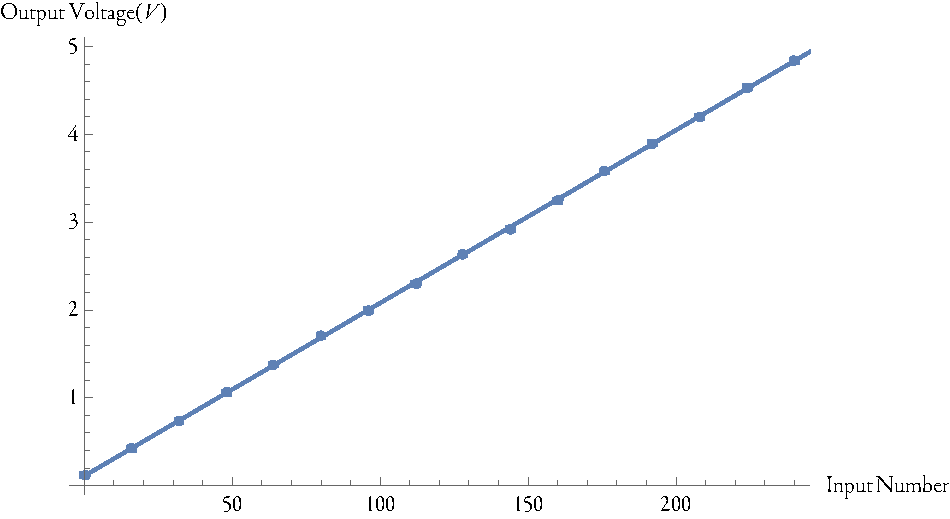
\includegraphics[height=1.8in]{plot.pdf}
% \end{center} 

%\begin{center}
% 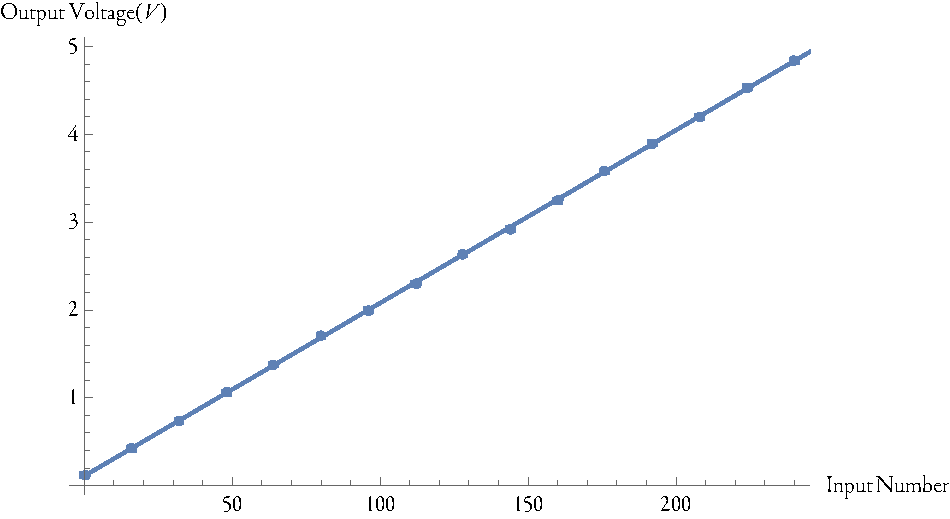
\includegraphics[height=1.3in]{plot.pdf}
%\end{center}

% \blindtext \cite{article-minimal}

% \bibliographystyle{apsrev4-1} % Tell bibtex which bibliography style to use
% \bibliography{xampl} % Tell bibtex which .bib file to use (this one is some example file in TexLive's file tree)

\end{document}